\chapter{相对论时空观}
\problem{考虑$2$维欧氏空间, 取一般坐标$\{u,v\}$, 与直角坐标关系为$x = x(u,v)$, $y = y(u,v)$. 求$2$维欧氏空间度规在$\{u,v\}$坐标下的形式.}
\begin{solution}
    由线元的定义, 我们有
    \begin{align*}
        \dd s^2 &= \left(\frac{\pp x}{\pp u} \dd u + \frac{\pp x}{\pp v} \dd v\right)^2 + \left(\frac{\pp y}{\pp u} \dd u + \frac{\pp y}{\pp v} \dd v\right)^2 \\
        &= \left(\frac{\pp x}{\pp u}\right)^2 \dd u^2 + \left(\frac{\pp x}{\pp v}\right)^2 \dd v^2 + 2\frac{\pp x}{\pp u} \frac{\pp x}{\pp v} \dd u \dd v + \left(\frac{\pp y}{\pp u}\right)^2 \dd u^2 + \left(\frac{\pp y}{\pp v}\right)^2 \dd v^2 + 2\frac{\pp y}{\pp u} \frac{\pp y}{\pp v} \dd u \dd v \\
        &= \begin{pmatrix}
            \dd u & \dd v
        \end{pmatrix} \begin{pmatrix}
            \left(\frac{\pp x}{\pp u}\right)^2+\left(\frac{\pp y}{\pp u}\right)^2 & \frac{\pp x}{\pp u} \frac{\pp x}{\pp v}+\frac{\pp y}{\pp u} \frac{\pp y}{\pp v} \\[0.8em]
            \frac{\pp x}{\pp u} \frac{\pp x}{\pp v}+\frac{\pp y}{\pp u} \frac{\pp y}{\pp v} & \left(\frac{\pp x}{\pp v}\right)^2+\left(\frac{\pp y}{\pp v}\right)^2
        \end{pmatrix} \begin{pmatrix}
            \dd u \\ \dd v
        \end{pmatrix}
    \end{align*}
    因此, 度规在$\{u,v\}$坐标下的形式为
    \[
        g_{ij} = \begin{pmatrix}
        	\left(\frac{\pp x}{\pp u}\right)^2+\left(\frac{\pp y}{\pp u}\right)^2 & \frac{\pp x}{\pp u} \frac{\pp x}{\pp v}+\frac{\pp y}{\pp u} \frac{\pp y}{\pp v} \\[0.8em]
        	\frac{\pp x}{\pp u} \frac{\pp x}{\pp v}+\frac{\pp y}{\pp u} \frac{\pp y}{\pp v} & \left(\frac{\pp x}{\pp v}\right)^2+\left(\frac{\pp y}{\pp v}\right)^2
        \end{pmatrix} 
    \]
\end{solution}

\problem{考虑$3$维欧氏空间, 已知球坐标与直角坐标的关系为$x = r \sin\theta \cos\phi$, $y = r \sin\theta \sin\phi$, $z = r \cos\theta$. 求$3$维欧氏空间度规在球坐标下的形式.}
\begin{solution}
    考虑$3$维欧氏空间中的矢量$\vec{v} = x \h{x} + y \h{y} + z \h{z}$, 由球坐标$\begin{cases}
            x = r \sin\theta \cos\phi \\
            y = r \sin\theta \sin\phi \\
            z = r \cos\theta
        \end{cases}$
    构造坐标系的坐标基矢
    \[
        \begin{aligned}
            \frac{\pp \vec{v}}{\pp r} &= \sin\theta \cos\phi \,\h{x} + \sin\theta \sin\phi \,\h{y} + \cos\theta \,\h{z} \\
            \frac{\pp \vec{v}}{\pp \theta} &= r \cos\theta \cos\phi \,\h{x} + r \cos\theta \sin\phi \,\h{y} - r \sin\theta \,\h{z} \\
            \frac{\pp \vec{v}}{\pp \phi} &= -r \sin\theta \sin\phi \,\h{x} + r \sin\theta \sin\phi \,\h{y}
        \end{aligned}
    \]
    则线元可以写为
    \begin{align*}
        \dd s^2 &= \dd \vec{v} \cdot \dd \vec{v} = g_{ij} \dd u^i \dd u^j\\
        &= \begin{pmatrix}
            \dd r & \dd \theta & \dd \phi
        \end{pmatrix} \begin{pmatrix}
            g_{rr} & g_{r\theta} & g_{\theta\phi} \\
            g_{\theta r} & g_{\theta\theta} & g_{\theta\phi} \\
            g_{\phi r} & g_{\phi\theta} & g_{\phi\phi}
        \end{pmatrix} \begin{pmatrix}
            \dd r \\ \dd \theta \\ \dd \phi
        \end{pmatrix}
    \end{align*}
    其中$g_{ij} = g_{ji} = \frac{\pp \vec{v}}{\pp u^i} \cdot \frac{\pp \vec{v}}{\pp u^j} =
    \frac{\pp x}{\pp u^i} \frac{\pp x}{\pp u^j} + \frac{\pp y}{\pp u^i}
    \frac{\pp y}{\pp u^j} + \frac{\pp z}{\pp u^i} \frac{\pp z}{\pp u^j}$.
    
    \vspace*{1em}
    由于坐标基矢正交, 即非对角元为零, 计算对角元得
    \begin{align*}
        g_{rr} &= \left(\frac{\pp x}{\pp r}\right)^2 + \left(\frac{\pp y}{\pp r}\right)^2 + \left(\frac{\pp z}{\pp r}\right)^2 = (\sin \theta \cos \phi)^2 + (\sin \theta \sin \phi)^2 + (\cos \theta)^2 = 1, \\
        g_{\theta\theta} &= \left(\frac{\pp x}{\pp \theta}\right)^2 + \left(\frac{\pp y}{\pp \theta}\right)^2 + \left(\frac{\pp z}{\pp \theta}\right)^2 = (r \cos \theta \cos \phi)^2 + (r \cos \theta \sin \phi)^2 + (-r \sin \theta)^2 = r^2, \\
        g_{\phi\phi} &= \left(\frac{\pp x}{\pp \phi}\right)^2 + \left(\frac{\pp y}{\pp \phi}\right)^2 + \left(\frac{\pp z}{\pp \phi}\right)^2 = (-r \sin \theta \sin \phi)^2 + (r \sin \theta \cos \phi)^2 = r^2 \sin^2\theta.
    \end{align*}

    将$g_{ij}$代入线元, 得
    \[
        \dd s^2 = \begin{pmatrix}
            \dd r & \dd \theta & \dd \phi
        \end{pmatrix} \begin{pmatrix}
            1 & 0 & 0 \\
            0 & r^2 & 0 \\
            0 & 0 & r^2 \sin^2\theta
        \end{pmatrix} \begin{pmatrix}
            \dd r \\ \dd \theta \\ \dd \phi
        \end{pmatrix}
    \]
    即$3$维欧氏空间度规在球坐标下的形式为
    \[
        g_{ij} = \begin{pmatrix}
            1 & 0 & 0 \\
            0 & r^2 & 0 \\
            0 & 0 & r^2 \sin^2\theta
        \end{pmatrix}
    \]
\end{solution}


\problem{如图\ref{fig:3-3}所示, $2$维环面参数方程为 $\begin{cases}
    x = (R + r \cos \theta) \cos \phi, \\
    y = (R + r \cos \theta) \sin \phi, \\
    z = r \sin \theta
\end{cases}$, 其中 $R$ 和 $r$ 是常数, $\{\theta, \phi\}$ 为环面的坐标, 取值为 $0$ 到 $2\pi$. 求$2$维环面的度规.}
\begin{figure}[h]
    \centering
    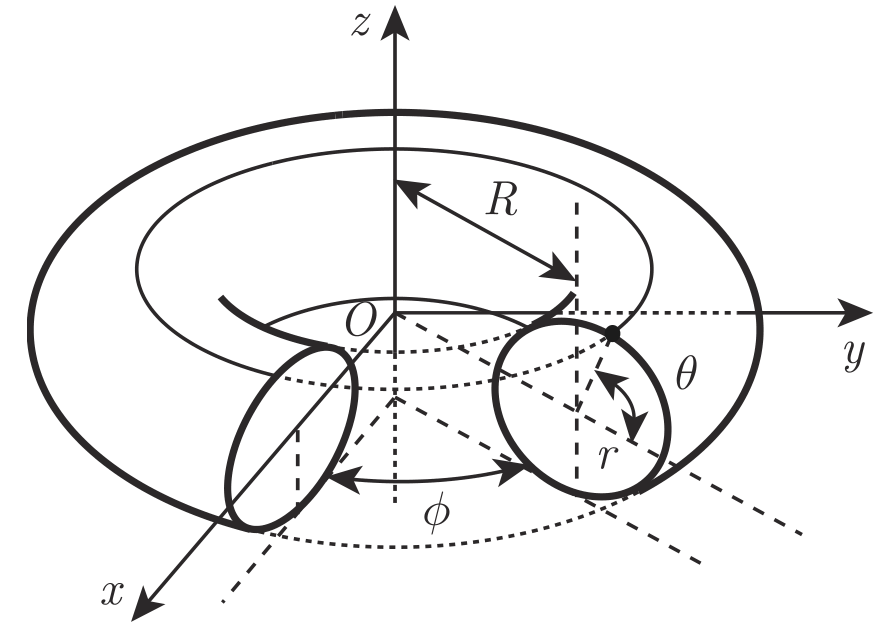
\includegraphics[width=0.3\textwidth]{content/Figures/3-3}
    \caption{ }
    \label{fig:3-3}
\end{figure}

\begin{solution}
	待写。
\end{solution}

\problem{某$2$维空间度规为$g_{ab}$,考虑(协变)矢量$V_a$、(逆变)矢量$A_a$、$2$阶张量$T_{ab}$。默认爱
	因斯坦求和约定,则下列表达式中,那些是有意义的,哪些是无意义的?对于有意义的表达式,写
	出其求和的具体展开式(例如: $V_a A^a = V_1 A^1 + V_2 A^2$)。(1) $V_a T_{ab}$;(2) $g^{ab}V_a$;(3) $g^{aa}$;(4)
	$A^a T_{ab}$;(5) $g^{ab}V_a T_{ab}$;(6) $g^{ab} V_b A^c T_{ac}$。}
	
\begin{solution}
	依据书上原话“需要强调,在引入了协变和逆变的概念后,所有的缩并一定是在一个上标和一个下标之间进行,
	而绝不会有两个上标或两个下标之间的缩并,也不会有多于两个的指标之间的缩并。”进行解答。\\
	(1)$V_a T_{ab}$对两个下标缩并,无意义;\\
	(2)$g^{ab}V_a$恰好是对一个上标和一个下标缩并,有意义,结果为
	\[g^{ab}V_a=g^{1b}V_1+g^{2b}V_2\]
	(3)$g^{aa}$出现两个相同的上标,无意义\footnote{存疑,为什么不能认为这个代表度规的对角元呢。};\\
	(4)$A^a T_{ab}$有意义,结果为
	\[A^a T_{ab}=A^1 T_{1b}+A^2 T_{2b}\]
	(5)$g^{ab}V_a T_{ab}$对于指标$a$,有多于两个的指标,无意义;\\
	(6)$g^{ab} V_b A^c T_{ac}$对于三组指标都是正确的,共有八项
	\begin{align*}
		g^{ab} V_b A^c T_{ac}&=g^{11} V_1 A^1 T_{11}+g^{11} V_1 A^2 T_{12}+g^{12} V_2 A^1 T_{11}+g^{12} V_2 A^2 T_{12}\\
		&+g^{21} V_1 A^1 T_{21}+g^{21} V_1 A^2 T_{22}+g^{22} V_2 A^1 T_{21}+g^{22} V_2 A^2 T_{22}
	\end{align*}
\end{solution}

\problem{已知闵氏时空中的洛伦兹变换为线性坐标变换\(x^\mu\to \tilde{x}^\mu={\Lambda^\mu}_\nu x^\nu\),其中\({\Lambda^\mu}_\nu\)为常矩
	阵。(1)验证若在洛伦兹变换下度规形式不变,则\({\Lambda^\mu}_\nu\)满足\(\eta_{\mu\nu}{\Lambda^\mu}_{\rho}{\Lambda^\nu}_{\sigma}=\eta_{\rho\sigma}\);( 2)考虑\(2\)维情形,度规为\(\eta_{\mu\nu}=\begin{pmatrix}-1 & 0\\ 0 & 1  \end{pmatrix}\),验证\({\Lambda^\mu}_\nu = \begin{pmatrix}\cosh{\beta} & \sinh{\beta}\\ \sinh{\beta} & \cosh{\beta}  \end{pmatrix}\)(\(\beta\)为常数)满足(1)的条件。}
	
\begin{solution}
	(1)考虑矢量的模长在洛伦兹变换下不变,即\(x^\mu x_\mu= \tilde{x}^\mu \tilde{x}_\mu\)或者写成
	\[\eta_{\mu\nu}x^\mu x^\nu=\eta_{\mu\nu}\tilde{x}^\mu \tilde{x}^\nu\]
	将\(\tilde{x}^\mu={\Lambda^\mu}_\nu x^\nu\)代入,
	\[\eta_{\mu\nu}x^\mu x^\nu=\eta_{\mu\nu}\tilde{x}^\mu \tilde{x}^\nu=\eta_{\mu\nu}{\Lambda^\mu}_\rho x^\rho {\Lambda^\nu}_\sigma x^\sigma=\eta_{\mu\nu}{\Lambda^\mu}_{\rho}{\Lambda^\nu}_{\sigma} x^\rho x^\sigma\]
	等式两边对照,即可得到\(\eta_{\mu\nu}{\Lambda^\mu}_{\rho}{\Lambda^\nu}_{\sigma}=\eta_{\rho\sigma}\)。
	
	(2)注意到\(\eta\)和\(\Lambda\)都是对称矩阵,于是其实等于验证\(\Lambda^T \eta \Lambda=\eta\),只需作矩阵乘法即可,也就是
	\begin{align*}
		\begin{pmatrix}\cosh{\beta} & \sinh{\beta}\\ \sinh{\beta} & \cosh{\beta}  \end{pmatrix}
		\begin{pmatrix}-1 & 0\\ 0 & 1  \end{pmatrix}
		\begin{pmatrix}\cosh{\beta} & \sinh{\beta}\\ \sinh{\beta} & \cosh{\beta}  \end{pmatrix}
		&=
		\begin{pmatrix}-\cosh{\beta} & \sinh{\beta}\\ -\sinh{\beta} & \cosh{\beta}  \end{pmatrix}
		\begin{pmatrix}\cosh{\beta} & \sinh{\beta}\\ \sinh{\beta} & \cosh{\beta}  \end{pmatrix}\\
		&=
		\begin{pmatrix}-\cosh^2{\beta}+\sinh^2{\beta} & 0\\ 0 & \cosh^2{\beta}-\sinh^2{\beta}  \end{pmatrix}\\
		&=
		\begin{pmatrix}-1 & 0\\ 0 & 1  \end{pmatrix}
	\end{align*}
	于是\(\Lambda^T \eta \Lambda=\eta\),验证完毕。
\end{solution}

\problem{考虑$4$维时空,已知闵氏度规$\eta_{\mu\nu}$及其逆$\eta^{\mu\nu}$满足$\eta^{\mu\rho}\eta_{\rho\nu}={\delta^\mu}_\nu$,这里${\delta^\mu	}_\nu$为单位矩阵。(1)求${\delta_\mu}^\nu$的矩阵形式;( 2)求${\eta^\mu}_\nu$的矩阵形式;(3)默认爱因斯坦求和约定,求${\eta^\mu}_\mu$和
	$\eta_{\mu\nu} \eta^{\mu\nu}$;(4)给定某矢量$A_\mu$,求$\frac{\partial A^\mu}{\partial A^\nu}$、$\frac{\partial A^\mu}{\partial A_\nu}$ $\frac{\partial A_\mu}{\partial A^\nu}$和$\frac{\partial A_\mu}{\partial A_\nu}$ ,用度规或单位矩阵表示出来(约定$\nu$为行指标,$\mu$为列指标);(5)定义$A^2=A_\mu A^\mu$,求$\frac{\partial A^2}{\partial A^\mu}$。( 6)求变分$\delta A$,用$\delta A_\mu$表示。}
	
\begin{solution}
	(1)可以直接计算得到\(\delta_{\mu\nu}=\eta_{\mu\sigma}{\delta^\sigma}_\nu=\eta_{\mu\nu}\),\({\delta_\mu}^\nu=\eta^{\nu\sigma}\delta_{\mu\sigma}=\eta^{\nu\sigma}\eta_{\mu\sigma}=\eta^{\nu\sigma}\eta_{\sigma\mu}={\delta^\nu}_\mu\),于是\({\delta_\mu}^\nu\)为单位矩阵,其矩阵形式为
	\begin{equation*}
		{\delta_\mu}^\nu=
		\begin{pmatrix}
			1 & 0 & 0 & 0\\
			0 & 1 & 0 & 0\\
			0 & 0 & 1 & 0\\
			0 & 0 & 0 & 1
		\end{pmatrix}
	\end{equation*}
	
	(2)直接计算\({\eta^\mu}_\nu=\eta^{\mu\sigma}\eta_{\sigma\nu}={\delta^\mu}_\nu\),为单位矩阵,其矩阵形式为
	\begin{equation*}
		{\eta^\mu}_\nu=
		\begin{pmatrix}
			1 & 0 & 0 & 0\\
			0 & 1 & 0 & 0\\
			0 & 0 & 1 & 0\\
			0 & 0 & 0 & 1
		\end{pmatrix}
	\end{equation*}
	
	(3)容易发现\({\eta^\mu}_{\mu}\)是对第(2)问中的矩阵求迹,结果为\({\eta^\mu}_{\mu}=4\)。而\(\eta_{\mu\nu} \eta^{\mu\nu}\)将所有元素平方求和,易得为\(\eta_{\mu\nu} \eta^{\mu\nu}=4\)。
	
	(4)逐个计算即可,对于不同的\(\mu\)和\(\nu\),\(A^\mu\)和\(A^\nu\)相互独立,于是\(\frac{\partial A^\mu}{\partial A^\nu}={\delta^\mu}_\nu\),\(\frac{\partial A^\mu}{\partial A_\nu}=\frac{\partial A^\mu}{\partial A^\sigma}\frac{\partial A^\sigma}{\partial A_\nu}={\delta^\mu}_\sigma \eta^{\sigma\nu}=\eta^{\mu\nu}\)。同理有\(\frac{\partial A_\mu}{\partial A^\nu}=\eta_{\mu\nu}\)和\(\frac{\partial A_\mu}{\partial A_\nu}={\delta_\mu}^\nu\)。
	
	(5)利用上一问的结论计算即可
	\[\frac{\partial(A^2)}{\partial A^\mu}=\frac{\partial(A_\nu A^\nu)}{\partial A^\mu}=A_\nu \frac{\partial A^\nu}{\partial A^\mu}+A^\nu \frac{\partial A_\nu}{\partial A^\mu}=A_\nu {\delta_\mu}^{\nu}+A^\nu \eta_{\mu \nu}=A_\mu+A_\mu=2 A_\mu\]
	
	(6)\(A=\sqrt{A^2}\),于是\(\delta A=\frac{A^\mu \delta A_\mu+A_\mu \delta A^\mu}{2 A}\),其中\(A_\mu \delta A^\mu=A_\mu \eta^{\mu\nu}\delta A_\nu=A^\nu \delta A_nu=A^\mu \delta A_mu\),回代,得
	\[\delta A=\frac{A^\mu }{A}\delta A_\mu\]
\end{solution}

\problem{考虑某 2 维空间,度规为 \( g_{ab}=\begin{pmatrix}g & 0\\ 0 & h \end{pmatrix}\),给定某矢量\(V_a=\begin{pmatrix}u \\ v\end{pmatrix}\)和某二阶张量 \( T_{ab}=\begin{pmatrix}a & b\\ c & d \end{pmatrix} \)。(1)求逆度规 \( g^{ab} \);(2)求 \( V^a,T^{ab},{T^a}_b,{T_a}^b \) 的矩阵形式;(3)利用上面的结果,写出 \( T_{ab}V^aV^b \)、\( T^{ab}V_aV_b \)、\( {T^a}_b V_aV^b \) 和 \( {T_a}^b V^a V_b \) 的具体矩阵表达式,并证明它们都相等。}

\begin{solution}
	(1)由于度规 \( g_{ab} \) 是对角矩阵,其逆度规 \( g^{ab} \) 为对角元素的倒数组成的对角矩阵:
	\[g^{ab} = \begin{pmatrix} \frac{1}{g} & 0 \\ 0 & \frac{1}{h} \end{pmatrix}\]
	
	(2)计算\( V^a \),只需通过度规升指标,\( V^a = g^{ab} V_b \)。计算得:
	\[V^a = g^{ab} V_b = \begin{pmatrix} \frac{1}{g} & 0 \\ 0 & \frac{1}{h} \end{pmatrix} \begin{pmatrix} u \\ v \end{pmatrix} = \begin{pmatrix} \dfrac{u}{g} \\[1em] \dfrac{v}{h} \end{pmatrix}\]
		计算\( T^{ab} \),只需通过度规升两个指标,\( T^{ab} = g^{ac} g^{bd} T_{cd} \)。计算得:
		\[T^{ab} = \begin{pmatrix} \dfrac{a}{g^2} & \dfrac{b}{g h} \\[1em] \dfrac{c}{g h} & \dfrac{d}{h^2} \end{pmatrix}\]
		计算\({T^a}_b\)只需根据\({T^a}_b=g^{ac}T_{cb}\),计算得到
		\[{T^a}_b=\begin{pmatrix}  \frac{a}{g} & \frac{b}{g} \\[1em] \frac{c}{h} & \frac{d}{h} \\ \end{pmatrix}\]
		计算\( {T_a}^b \)只需注意到\( {T_a}^{b} = g^{bc} T_{ac} \)。计算得:
		\[{T_a}^{b} = \begin{pmatrix} \dfrac{a}{g} & \dfrac{b}{h} \\[1em] \dfrac{c}{g} & \dfrac{d}{h} \end{pmatrix}\]
		其中矩阵的行对应下标 \( a \),列对应上标 \( b \)。
		
	(3)暴力计算即可,计算得到
	\begin{align*}
		T_{ab}V^aV^b&=\frac{a u^2}{g^2}+\frac{b u v}{g h}+\frac{c u v}{g h}+\frac{d v^2}{h^2}\\
		T^{ab}V_aV_b&=\frac{a u^2}{g^2}+\frac{b u v}{g h}+\frac{c u v}{g h}+\frac{d v^2}{h^2}\\
		{T^a}_b V_aV^b&=\frac{a u^2}{g^2}+\frac{b u v}{g h}+\frac{c u v}{g h}+\frac{d v^2}{h^2}\\
		{T_a}^b V^a V_b&=\frac{a u^2}{g^2}+\frac{b u v}{g h}+\frac{c u v}{g h}+\frac{d v^2}{h^2}
	\end{align*}
\end{solution}
